\begin{proofbox}
\textbf{\textcolor{CProof}{先把“为什么有这条线”证明出来，再证明“互换关系”}}

本节给出四种证明路径：\textbf{方法一门槛最低}（只用勾股定理、展开与交换律），\textbf{方法二考场速度最快}（直接看标准方程），\textbf{方法三书写步骤最少}（一个共同等式），\textbf{方法四常规通用}（展开一般二次方程）。学生先掌握前两种即可；最后一种用于检验较一般的曲线方程，不作为入门要求。

\medskip
\textbf{\textcolor{CProof}{预备：为什么圆外点的切点弦满足 $x_1x+y_1y=r^2$？}}

设圆 $x^2+y^2=r^2$，圆心 $O(0,0)$，圆外一点 $P(x_1,y_1)$ 满足 $x_1^2+y_1^2>r^2$。从 $P$ 向圆作切线，设其中一个切点为 $T(x,y)$。

\begin{center}
\begin{tikzpicture}[x=1.2cm,y=1.2cm,every node/.style={font=\small}]
\coordinate (O) at (0,0); \coordinate (P) at (4,0);
\coordinate (T) at (1,{sqrt(3)}); \coordinate (U) at (1,{-sqrt(3)});
\draw[blue!75!black,thick] (O) circle (2);
\draw[gray!70] (O)--(P) (O)--(U);
\draw[orange!80!black,thick] (P)--(T) (P)--(U);
\draw[gray!80,thick] (O)--(T) node[midway,above left] {$r$};
\draw[red!75!black,dashed,thick] (1,-2.2)--(1,2.3);
\draw ($(T)!.16!(O)$)--($(T)!.16!(O)+(.277128,-.16)$)--($(T)+(.277128,-.16)$);
\fill (O) circle (1.8pt) node[below left] {$O$};
\fill (P) circle (2pt) node[below right] {$P$};
\fill (T) circle (2pt) node[above right] {$T(x,y)$};
\fill (U) circle (2pt) node[below right] {$T'$};
\node[red!75!black,above] at (1,2.3) {$l_P=TT'$};
\node at (1,-2.9) {$OT\perp PT\quad\Longrightarrow\quad OP^2=OT^2+PT^2$};
\end{tikzpicture}

\end{center}
图取 $r=2,P(4,0)$ 展示构造；下文仍用任意 $r,P$ 推导。要用的是 $T$ 处的直角。
\begin{description}[style=nextline,leftmargin=2.8em,itemsep=0.42em]
\item[\textbf{第一步：写出三条线段的长度平方。}] 因为 $T$ 在圆上，$OT^2=x^2+y^2=r^2$；$OP^2=x_1^2+y_1^2$；用两点距离公式得 $PT^2=(x-x_1)^2+(y-y_1)^2$。
\item[\textbf{第二步：使用切线与半径垂直。}] 切点处 $OT\perp PT$，所以直角三角形 $OTP$ 满足
\[
OP^2=OT^2+PT^2.
\]
代入三段长度：
\[
x_1^2+y_1^2=r^2+(x-x_1)^2+(y-y_1)^2.
\]
\item[\textbf{第三步：展开，不跳步。}] 右边展开为
\[
r^2+x^2-2xx_1+x_1^2+y^2-2yy_1+y_1^2.
\]
两边同时减去 $x_1^2+y_1^2$，得到
\[
0=r^2+x^2+y^2-2xx_1-2yy_1.
\]
再由 $x^2+y^2=r^2$，得到 $0=2r^2-2xx_1-2yy_1$，从而
\[
\boxed{x_1x+y_1y=r^2}.
\]
\item[\textbf{第四步：解释整条线。}] 另一个切点也满足同一等式，因此两切点都在直线 $x_1x+y_1y=r^2$ 上；两个切点不重合，所以这条直线\textbf{正是切点弦所在的直线}。当 $P$ 移到圆上时，相同方程变成 $P$ 处的切线；当 $P$ 在圆内且 $P\ne O$ 时，相同方程仍定义一条直线，却不代表真实切点弦。
\end{description}

\medskip
\textbf{\textcolor{CProof}{方法一：门槛最低——从圆的互换式开始}}


\begin{center}
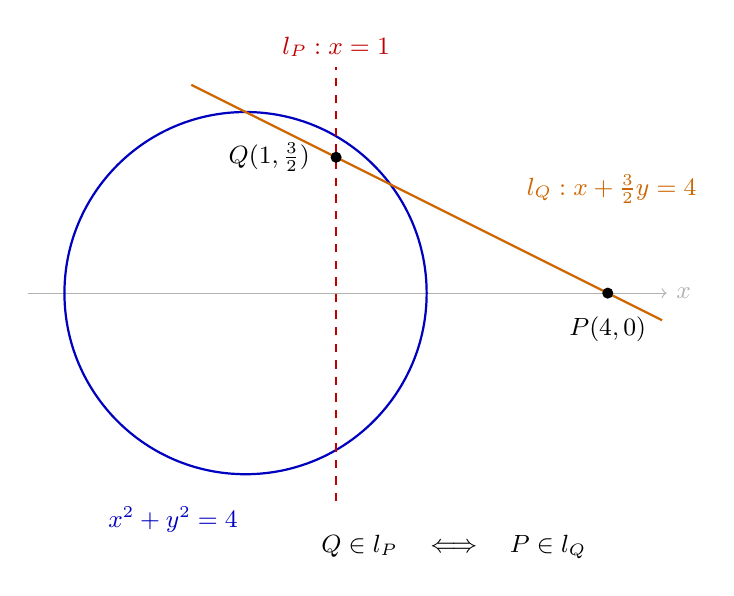
\begin{tikzpicture}[x=1.15cm,y=1.15cm,every node/.style={font=\small}]
\draw[->,gray!60] (-2.4,0)--(4.65,0) node[right] {$x$};
\draw[blue!75!black,thick] (0,0) circle (2);
\draw[red!75!black,thick,dashed] (1,-2.3)--(1,2.5);
\draw[orange!80!black,thick] (-.6,2.3)--(4.6,-.3);
\fill (4,0) circle (2pt) node[below=5pt] {$P(4,0)$};
\fill (1,1.5) circle (2pt) node[left=6pt] {$Q(1,\frac32)$};
\node[red!75!black,above] at (1,2.5) {$l_P:x=1$};
\node[orange!80!black,right] at (3,1.15) {$l_Q:x+\frac32y=4$};
\node[blue!75!black] at (-.8,-2.5) {$x^2+y^2=4$};
\node at (2.3,-2.8) {$Q\in l_P\quad\Longleftrightarrow\quad P\in l_Q$};
\end{tikzpicture}

\end{center}
图中取 $P(4,0),Q(1,\frac32)$：分别代入对方的直线，两次检验同为 $4$。

设 $P(x_1,y_1),Q(x_2,y_2)$ 都不是圆心。对圆 $x^2+y^2=r^2$：
\begin{description}[style=nextline,leftmargin=2.8em,itemsep=0.42em]
\item[\textbf{第一步：写出 $P$ 的极线。}] $l_P:x_1x+y_1y=r^2$。这个方程中的 $x,y$ 是\textbf{直线上任意点的坐标}，$x_1,y_1$ 才是固定点 $P$ 的坐标。
\item[\textbf{第二步：把 $Q$ 放进去。}] $Q$ 在 $l_P$ 上，当且仅当
\[x_1x_2+y_1y_2=r^2.\]
\item[\textbf{第三步：反过来写 $Q$ 的极线。}] $l_Q:x_2x+y_2y=r^2$，$P$ 在其中当且仅当
\[x_2x_1+y_2y_1=r^2.\]
\item[\textbf{第四步：比较。}] $x_1x_2=x_2x_1$，$y_1y_2=y_2y_1$。两式完全相同，所以 $Q\in l_P\iff P\in l_Q$。
\end{description}
\textbf{补足圆上点的理解：} 若点 $P(u,v)$ 本身在圆上，即 $u^2+v^2=r^2$，那么 $P$ 显然满足 $ux+vy=r^2$。设圆上另一个点 $X(x,y)$ 也在此直线上，则
\[
\begin{aligned}
PX^2&=(x-u)^2+(y-v)^2\\
&=(x^2+y^2)+(u^2+v^2)-2(ux+vy)\\
&=r^2+r^2-2r^2=0.
\end{aligned}
\]
所以 $X$ 只能与 $P$ 重合。这说明该直线与圆\textbf{只有一个公共点 $P$}，就是圆在 $P$ 处的切线。这里既没有用导数，也没有用新理论。

\textbf{几何意义：} 你把“点在线上”的条件交换一下说法，既没有增加条件，也没有减少条件。这才是本结论的全部核心。

\medskip
\textbf{\textcolor{CProof}{方法二：速度最快——看三个标准方程的左右两边}}


\begin{center}
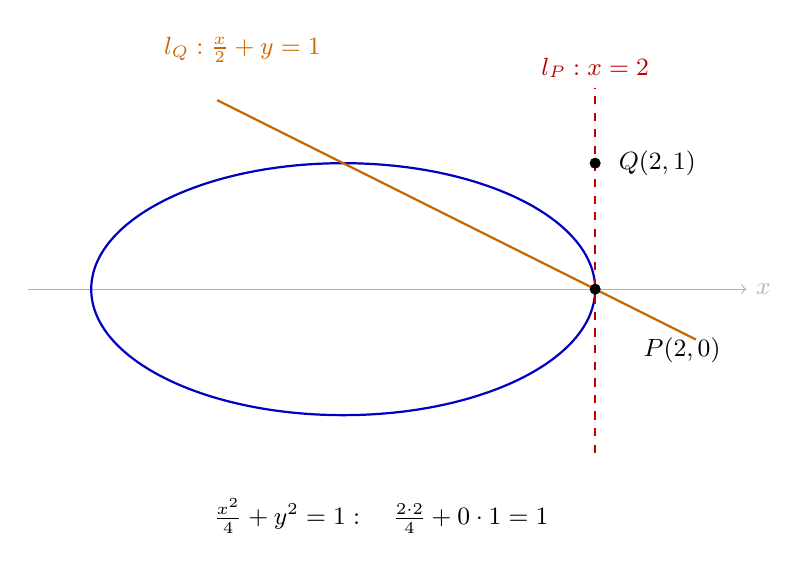
\begin{tikzpicture}[x=1.6cm,y=1.6cm,every node/.style={font=\small}]
\draw[->,gray!60] (-2.5,0)--(3.2,0) node[right] {$x$};
\draw[blue!75!black,thick] (0,0) ellipse (2 and 1);
\draw[red!75!black,dashed,thick] (2,-1.3)--(2,1.6);
\draw[orange!80!black,thick] (-1,1.5)--(2.8,-.4);
\fill (2,0) circle (2pt) node[below right=14pt] {$P(2,0)$};
\fill (2,1) circle (2pt) node[right=5pt] {$Q(2,1)$};
\node[red!75!black,above] at (2,1.6) {$l_P:x=2$};
\node[orange!80!black] at (-.8,1.9) {$l_Q:\frac{x}{2}+y=1$};
\node at (.3,-1.8) {$\frac{x^2}{4}+y^2=1:\quad \frac{2\cdot2}{4}+0\cdot1=1$};
\end{tikzpicture}

\end{center}
先用椭圆实例看清：$Q$ 在竖直的 $l_P$ 上，$P$ 在斜的 $l_Q$ 上。下面比较标准方程中的检验式。

对于下面三种曲线，只需把\textbf{点 $Q$ 代入点 $P$ 对应的直线}，观察所得等式：
\begin{description}[style=nextline,leftmargin=2.8em,itemsep=0.42em]
\item[\textbf{椭圆：}] 设 $\frac{x^2}{a^2}+\frac{y^2}{b^2}=1\;(a>b>0)$。$l_P:\frac{x_1x}{a^2}+\frac{y_1y}{b^2}=1$；所以
\[
Q\in l_P\iff \frac{x_1x_2}{a^2}+\frac{y_1y_2}{b^2}=1.
\]
交换 $1,2$ 的顺序并不改变算式，所以这一条件正好等价于 $P\in l_Q$。
\item[\textbf{双曲线：}] 设 $\frac{x^2}{A^2}-\frac{y^2}{B^2}=1\;(A,B>0)$。相应的判断式为
\[
Q\in l_P\iff \frac{x_1x_2}{A^2}-\frac{y_1y_2}{B^2}=1.
\]
这里虽然有减号，但每一项的乘法顺序仍可交换，结论不变。
\item[\textbf{抛物线：}] 设 $y^2=2px\;(p>0)$。由 $l_P:y_1y=p(x+x_1)$，得
\[
Q\in l_P\iff y_1y_2=p(x_1+x_2).
\]
把 $1,2$ 互换，左侧是相同的乘积，右侧是相同的和，仍等价于 $P\in l_Q$。
\end{description}
\textbf{考场思路：} 不必把极线两边都完整求出来；写出一次“两个点的坐标共同满足的等式”，就能看出是否可交换。

\medskip
\textbf{\textcolor{CProof}{方法三：步骤最少——两条直线共同使用同一判断式}}


\begin{center}
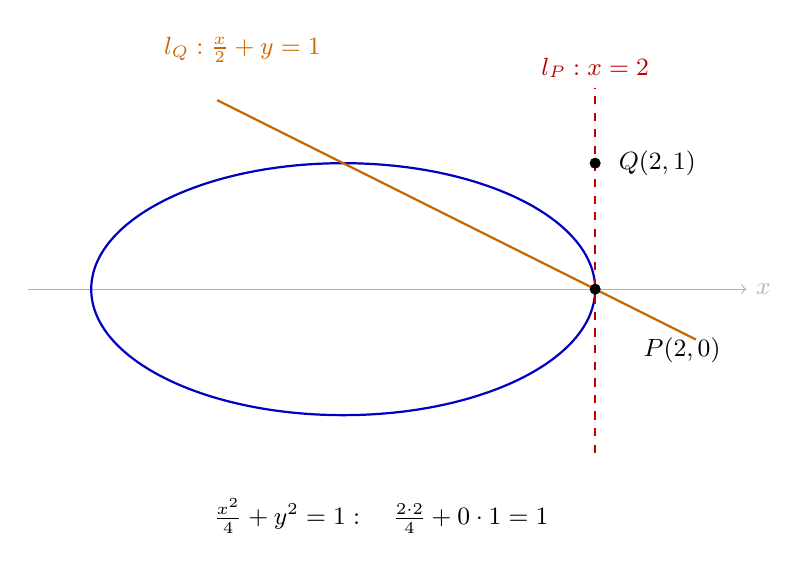
\begin{tikzpicture}[x=1.6cm,y=1.6cm,every node/.style={font=\small}]
\draw[->,gray!60] (-2.5,0)--(3.2,0) node[right] {$x$};
\draw[blue!75!black,thick] (0,0) ellipse (2 and 1);
\draw[red!75!black,dashed,thick] (2,-1.3)--(2,1.6);
\draw[orange!80!black,thick] (-1,1.5)--(2.8,-.4);
\fill (2,0) circle (2pt) node[below right=14pt] {$P(2,0)$};
\fill (2,1) circle (2pt) node[right=5pt] {$Q(2,1)$};
\node[red!75!black,above] at (2,1.6) {$l_P:x=2$};
\node[orange!80!black] at (-.8,1.9) {$l_Q:\frac{x}{2}+y=1$};
\node at (.3,-1.8) {$\frac{x^2}{4}+y^2=1:\quad \frac{2\cdot2}{4}+0\cdot1=1$};
\end{tikzpicture}

\end{center}
仍看同一椭圆构型；本方法只抓住图下的共同等式，不重复求两条直线。

以椭圆为例，直接写
\[
\begin{aligned}
Q\in l_P
&\iff \frac{x_1x_2}{a^2}+\frac{y_1y_2}{b^2}=1\\
&\iff \frac{x_2x_1}{a^2}+\frac{y_2y_1}{b^2}=1\\
&\iff P\in l_Q.
\end{aligned}
\]
这三行就是完整证明。圆、双曲线将中间式中的系数和符号换成对应标准形式即可。抛物线则用 $y_1y_2=p(x_1+x_2)$，证明同样只有三行。

\textbf{特别提醒：} 这不是凭空把 $P,Q$ 互换。\textbf{因为对应直线的方程本来就有这个交换后不变的结构}，所以互换才合法。

\medskip
\par\noindent\begin{minipage}{\linewidth}
\textbf{\textcolor{CProof}{方法四：常规通用——一般二次方程逐项展开}}

这一方法只用高中代数运算，但式子长。想理解“上面为什么都能统一”时再读。


\begin{center}
\begin{tikzpicture}[x=1.5cm,y=1.5cm,every node/.style={font=\small}]
\draw[->,gray!60] (-2.3,0)--(3,0) node[right] {$x$};
\draw[blue!75!black,thick,rotate=-45] (0,0) ellipse ({sqrt(6)} and {sqrt(2)});
\draw[red!75!black,dashed,thick] (.3,2.4)--(2.5,-2);
\draw[orange!80!black,thick] (-.3,2.3)--(2.7,-.7);
\fill (2,0) circle (2pt);\node at (2.8,-1.2) {$P(2,0)$};
\fill (1,1) circle (2pt) node[right=6pt] {$Q(1,1)$};
\node[red!75!black,above] at (.3,2.4) {$l_P:2x+y=3$};
\node[orange!80!black,right] at (2.4,.5) {$l_Q:x+y=2$};
\node at (.2,-2.5) {$x^2+xy+y^2=3$（含交叉项 $xy$）};
\end{tikzpicture}

\end{center}
\end{minipage}\par
具体实例中，$\alpha=\gamma=1,\beta=1,\delta=\varepsilon=0,\varphi=-3$。代入 $P,Q$ 得 $U=2+1-3=0$；反向代入也为 $0$，交叉项没有破坏互换。

设曲线的方程为
\[
S(x,y)=\alpha x^2+\beta xy+\gamma y^2+\delta x+\varepsilon y+\varphi=0.
\]
其中系数是固定的。只考虑这个方程确实表示通常的一条二次曲线，而且下面给出的直线方程不是 $0=0$ 或 $0=\text{非零常数}$ 的情况。为点 $P(x_1,y_1)$ 配出下面的直线：
\[
\begin{aligned}
l_P:\quad &\alpha x_1x+\frac{\beta}{2}(x_1y+y_1x)+\gamma y_1y\\
&+\frac{\delta}{2}(x_1+x)+\frac{\varepsilon}{2}(y_1+y)+\varphi=0.
\end{aligned}
\]
为什么系数里出现一半？因为像 $xy$ 这样的项需要平均写成 $\frac12(x_1y+y_1x)$，这样\textbf{把两点交换时不会偏向其中一个点}；而 $x$ 则平均写成 $\frac12(x_1+x)$。对标准的圆、椭圆、双曲线、抛物线，把它们的系数代入就能还原前面已经用过的简单公式。

把 $Q(x_2,y_2)$ 代入 $l_P$ 的左边，所得数为
\[
\begin{aligned}
U={}&\alpha x_1x_2+\frac{\beta}{2}(x_1y_2+y_1x_2)+\gamma y_1y_2\\
&+\frac{\delta}{2}(x_1+x_2)+\frac{\varepsilon}{2}(y_1+y_2)+\varphi.
\end{aligned}
\]
反过来，把 $P$ 代入 $Q$ 的极线，所得数为
\[
\begin{aligned}
V={}&\alpha x_2x_1+\frac{\beta}{2}(x_2y_1+y_2x_1)+\gamma y_2y_1\\
&+\frac{\delta}{2}(x_2+x_1)+\frac{\varepsilon}{2}(y_2+y_1)+\varphi.
\end{aligned}
\]
逐项比较：
\[
\begin{array}{rcl}
 x_1x_2&=&x_2x_1,\\
 x_1y_2+y_1x_2&=&y_2x_1+x_2y_1,\\
 y_1y_2&=&y_2y_1,\\
 x_1+x_2&=&x_2+x_1,\\
 y_1+y_2&=&y_2+y_1.
\end{array}
\]
所以 $U=V$，特别是 $U=0\iff V=0$，即
\[
\boxed{Q\in l_P\iff P\in l_Q}.
\]
\textbf{看懂本方法只需要两句话：} 第一，把一个点放进另一个点对应的直线，得到一个具体算式；第二，交换两点后，算式完全不变。

\medskip
\textbf{\textcolor{CProof}{附证明：为什么它能找出动直线的定点？}}


\begin{center}
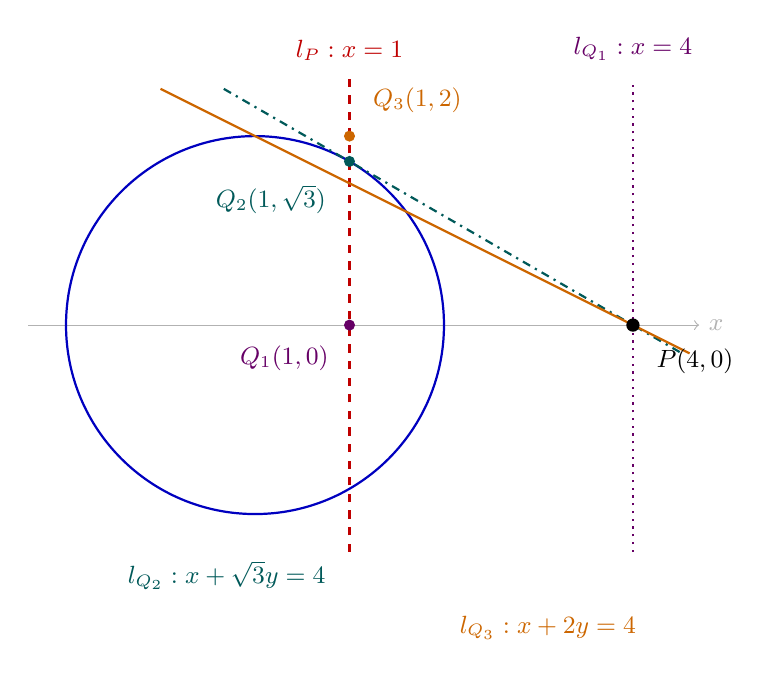
\begin{tikzpicture}[x=1.2cm,y=1.2cm,every node/.style={font=\small}]
\draw[->,gray!60] (-2.4,0)--(4.7,0) node[right] {$x$};
\draw[blue!75!black,thick] (0,0) circle (2);
\draw[red!75!black,dashed,thick] (1,-2.4)--(1,2.6);
\draw[violet!80!black,thick,dotted] (4,-2.4)--(4,2.6);
\draw[teal!70!black,thick,dash dot] ({4-2.5*sqrt(3)},2.5)--(4.5,{-0.5/sqrt(3)});
\draw[orange!80!black,thick] (-1,2.5)--(4.6,-.3);
\fill (4,0) circle (2.4pt) node[below right=5pt] {$P(4,0)$};
\fill[violet!80!black] (1,0) circle (2pt) node[below left=4pt] {$Q_1(1,0)$};
\fill[teal!70!black] (1,{sqrt(3)}) circle (2pt) node[below left=5pt] {$Q_2(1,\sqrt3)$};
\fill[orange!80!black] (1,2) circle (2pt) node[above right=5pt] {$Q_3(1,2)$};
\node[red!75!black,above] at (1,2.7) {$l_P:x=1$};
\node[violet!80!black,above] at (4,2.7) {$l_{Q_1}:x=4$};
\node[teal!70!black] at (-.3,-2.65) {$l_{Q_2}:x+\sqrt3y=4$};
\node[orange!80!black] at (3.1,-3.2) {$l_{Q_3}:x+2y=4$};
\end{tikzpicture}

\end{center}
观察三种 $Q$：对应直线的位置不同，但交在同一个 $P$。下文验证任意参数，而非仅验证图中三条线。

只用方法一的圆，取 $P(4,0)$，那么 $l_P:x=1$。令 $Q(1,t)$ 在这条直线上移动，得到 $l_Q:x+ty=4$。由于任意 $t$ 都有
\[
\underbrace{4}_{x_P}+t\underbrace{\cdot0}_{y_P}=4,
\]
所以 $P(4,0)$ 在每一条 $l_Q$ 上。这就是前面互换结论的实际用途。

\textbf{如果不预先知道定点在哪里，也能直接求：} 设有一点 $(u,v)$ 在所有 $x+ty=4$ 上；取 $t=0$ 得 $u=4$；再取 $t=1$ 得 $u+v=4$，所以 $v=0$。定点唯一为 $(4,0)$。极线方法的优势，是它让我们\textbf{在展开之前就能预料到这个点在哪里}。
\end{proofbox}
